\chapter{Practical Applications} \label{cha:practical-appl}

We will now apply the concept of shape-constraint P-splines onto real-world data to incorporated a priori domain knowledge into the modeling process. In the first example, see~\pref{sec:real-world-application}, we use the domain knowledge to enhance the estimation of the heat transfer coefficient in a heat-treatment process. The main challenge here is the sparse and noisy data situation combined with a highly non-linear process. In the second example, see~\pref{sec:real-world-application2}, we investigate the behavior of a servo-compensation which possesses a discontinuity as main challenge.  

\section{Parameter Estimation} \label{sec:real-world-application}

The data is generated from a heat-treatment process of aluminum strips. The aluminum strip is heated up to a specific temperature, hold at this temperature for some predefined time and then rapidly cooled down to room temperature by means of water jets. The controlled heating and cooling enhances structural properties of the aluminum strip.

The area of interest is the cooling phase of the strip, in which some highly non-linear processes take place due to phase transitions of the cooling medium water. The temperature evolution T of the strip mainly depends on the heat transfer coefficient $\alpha$ characterizing the interaction between the aluminum strip and water. A complete description of the physical effects during water cooling is still research. Therefore, modeling of the heat transfer coefficient using first-principle methods is not expedient. Nevertheless, we can use the first-principle ideas in the form of a priori domain knowledge. To describe the temperature evolution during the cooling phase, we try to estimate the heat transfer coefficient, i.e.

\begin{align}
	\alpha := \alpha(T, \dot m),
\end{align}
%
as a function of the temperature $T$ of the aluminum strip and the mass flow $\dot m$ of the cooling medium. We know beforehand, that the heat transfer coefficient $\alpha$ may only increase with increasing mass flow $\dot m$ and that it shows unimodal peak behavior for increasing temperature $T$, motivated by the so-called Leidenfrost effect, see \cite{mayinger2013stromung} and \cite{baehr2006heatandmasstransfer}.

The data is determined by elaborate experiments performed on a prototype of Ebner Industrieofenbau. The distribution of data is visualized in~\pref{fig:ebner_data_situation}. Here we show how many data points are given in a square area of approximately 50 $\si{K}$ and 0.9 $\si{kg}/\si{s}$, which represent approximately 1\% of the whole input space. We have some regions, where no data is available, while the majority of data points is located in small areas, see~\pref{sec:peak-behav-sparse}. This problem, i.e. of irregular data distribution, is often encountered in real-world situations. 

\begin{figure}[H]
	\centering
	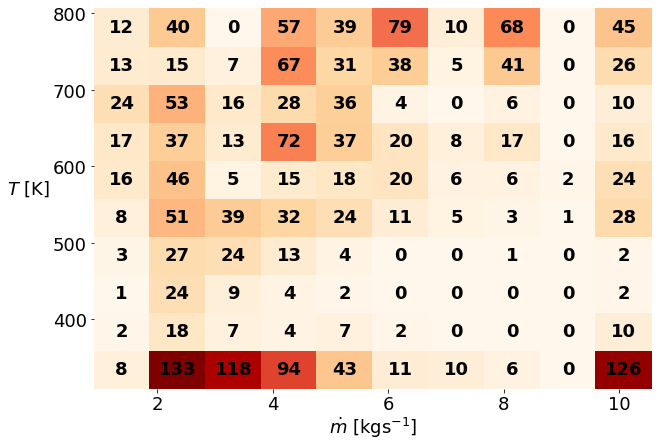
\includegraphics[width=0.8\columnwidth]{graphics/pgfplots/cha5/Ebner/data_distribution.png}
	\caption{Data distribution.}
	\label{fig:ebner_data_situation}
\end{figure}

The data distribution may lead to some difficulties when using B-splines and tensor-product B-splines, as they do not handle sparse data situations well, cf.~\pref{cha:practical-considerations}. Nevertheless, using regularization via smoothness and constraint penalties should help to cope with the data situation. 

We will now use various models based on B-spline bases, tensor-product B-spline bases and their shape-constraint alternatives to recover a model for the heat transfer coefficient given the data. The following list, in which $s(x_i)$ denotes the use of a B-spline basis for input $x_i \in \{\dot{m}, T\}$ and $t(\dot{m}, T)$ denotes the use of a tensor-product B-spline basis, describes the models that are analyzed. 

\begin{enumerate}[(i)]
	\item M1 $= s(\dot{m}) + s(T)$ without constraints
	\item M2 $= s(\dot{m}) + s(T)$, with monotonicity for $s(\dot{m})$ and unimodal peak behavior for $s(T)$
	\item M3 $= t(\dot{m}, T)$ without constraints
	\item M4 $= t(\dot{m}, T)$, wiht monotonicity for input $1$
	\item M5 $= s(\dot{m}) + s(T) + t(\dot{m}, T)$, as additive model without constraints
	\item M6 $= s(\dot{m}) + s(T) + t(\dot{m}, T)$, as additive model with constraints defined in M2 and M4
\end{enumerate}
%
Note that we use a smoothness penalty optimized via generalized cross-validation for each individual basis. The unconstraint models M1, M3 and M5 are therefore P-spline models rather than B-spline models. The shape-constraint models M2, M4 and M6 are SCP-spline models. 


To fit the models listed above, we perform a randomized train-validation split on the data, i.e. we split the data into a training set $\mathcal{D}_{\text{train}}$ and a validation set $\mathcal{D}_{\text{val}}$, fit the models to the resulting training set and evaluate its performance by calculating the mean squared error MSE, see~\pref{eq:MSE-DEF}, on the validation set $\mathcal{D}_{\text{val}}$ and the effective degree of freedom EDoF of the model, see~\pref{eq:EDoF}, as well as by visual inspection. We choose to split the data into sets of the same size to generate a more stable estimation of the prediction error for previously unseen data. A visual inspection of the of the data distribution given by the train-validation split is given in~\pref{fig:ebner-train-val-split}.

\begin{figure}[H]
	\centering
	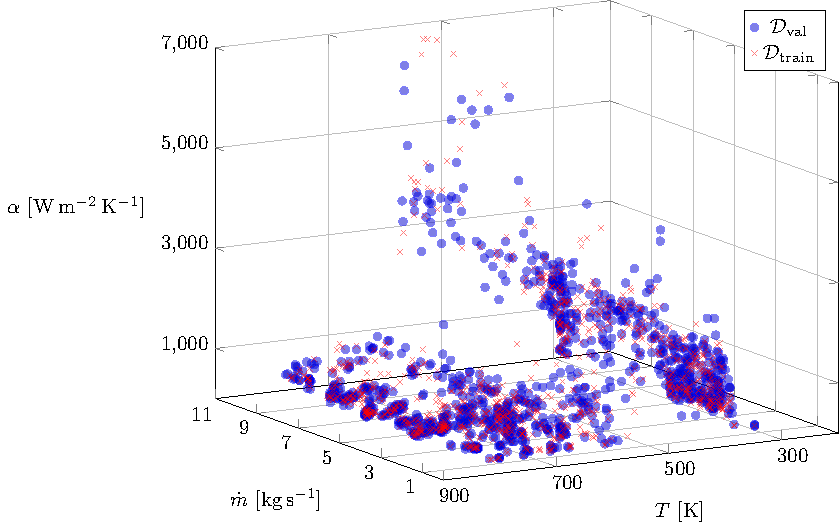
\includegraphics[width=\columnwidth]{graphics/pgfplots/cha5/Ebner/train-val-split.pdf}
	\caption{Validation set $\mathcal{D}_{\text{val}}$ and training set $\mathcal{D}_{\text{train}}$.}
	\label{fig:ebner-train-val-split}
\end{figure}
%

The mean squared errors $\mathrm{MSE}_{\mathrm{val}}$ evaluated on the validations set $\mathcal{D}_{\text{val}}$ as well as the effective degree of freedom EDoF of the models are given in~\pref{tab:ebner-mse-val}. According to these, the best model is M4, i.e. the shape-constraint tensor-product B-spline with a monotonicity constraint in the mass flow dimension. The models M3, i.e. the tensor-product B-spline, and M6, i.e. the additive model using shape-constraints, perform nearly as well as M4 according to the mean squared error on the validation set but both possess a significantly higher EDoF which allows for some overfitting. 

\begin{table}[H]
	\begin{center}
		\pgfplotstabletypeset[
		col sep=comma,
		columns/Model/.style={string type},
		columns/MSE_val/.style={column name={$\text{MSE}_{\text{val}}$}},
		every head row/.style={before row=\toprule[1pt] \toprule,after row=\midrule[2pt]},
		every last row/.style={after row=\bottomrule \bottomrule},
		every nth row={1}{before row=\midrule},
		]{graphics/data/cha5/Ebner/mses.csv}
	\end{center}
	\caption{Mean squared errors on the validation set $\mathcal{D}_{\text{val}}$ and effective degree of freedom EDoF of the models.}
	\label{tab:ebner-mse-val}
\end{table}

The predictions for model M4 are shown in~\pref{fig:ebner-M4}. The peak behavior in the temperature dimension is clearly visible, as well as an increasing trend within the mass flow dimension. Therefore, we conclude that model M4 is the superior model with regards to the domain knowledge and data fidelity. 

\begin{figure}[H]
	\centering
	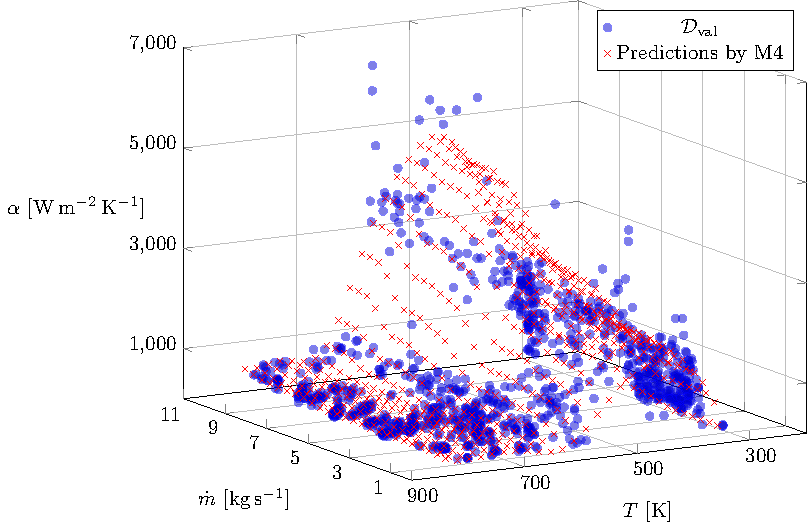
\includegraphics[width=\columnwidth]{graphics/pgfplots/cha5/Ebner/M4.pdf}
	\caption{Validation set $\mathcal{D}_{\text{val}}$ and predictions by model M4.}
	\label{fig:ebner-M4}
\end{figure}

The predictions for model M6 are shown in~\pref{fig:ebner-M6}. Here, the peak behavior can also be identified, but in a weaker fashion as for model M4 in~\pref{fig:ebner-M4}. We also obtain an increasing trend in the mass flow dimension. 

\begin{figure}[H]
	\centering
	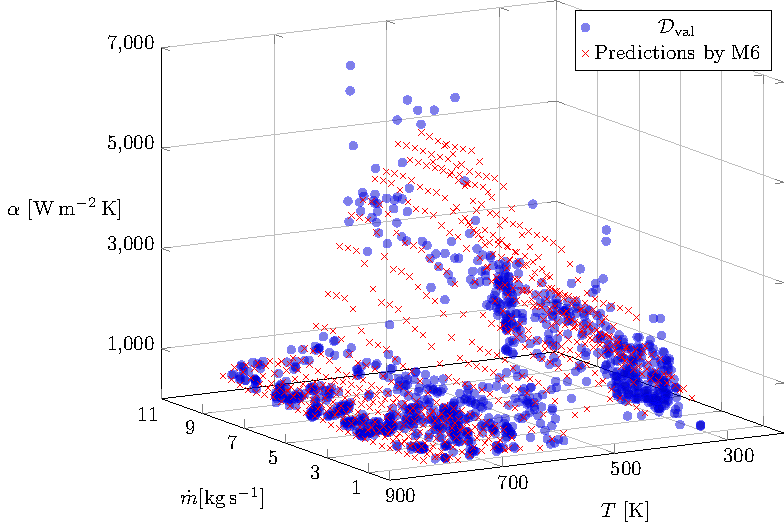
\includegraphics[width=\columnwidth]{graphics/pgfplots/cha5/Ebner/M6.pdf}
	\caption{Validation set $\mathcal{D}_{\text{val}}$ and predictions by model M6.}
	\label{fig:ebner-M6}
\end{figure}
%
The visual inspection of the predictions of model M3 in~\pref{fig:ebner-M3} indicates that there is massive overfitting present. Neither smooth, nor the a priori known behavior (increasing in the mass flow dimension and a peak behavior in the temperature dimension) is identifiable.  

\begin{figure}[H]
	\centering
	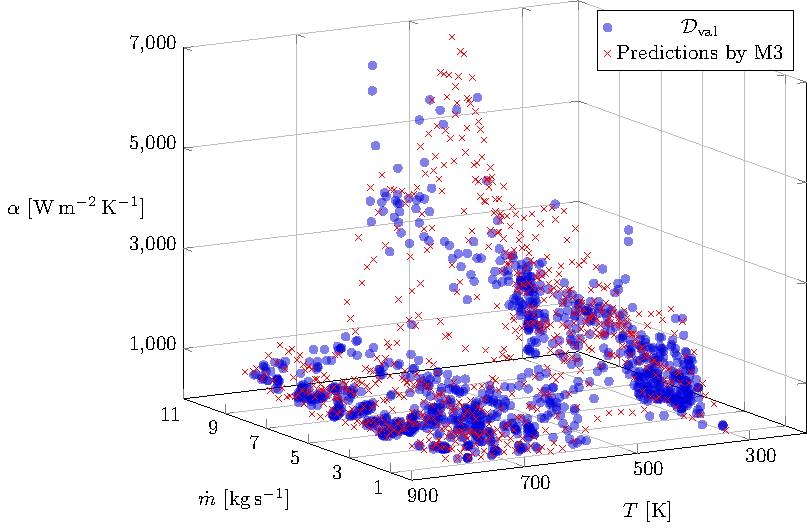
\includegraphics[width=\columnwidth]{graphics/pgfplots/cha5/Ebner/M3.pdf}
	\caption{Validation set $\mathcal{D}_{\text{val}}$ and predictions by model M3.}
	\label{fig:ebner-M3}
\end{figure}

We omit the visual presentation of the predictions by the models M1, M2 and M5, since for all of these the metrics, mean squared errors on the validation set $\mathcal{D}_{\text{val}}$ and the effective degree of freedom EDoF, indicate even worse models.

To summarized, we see that the incorporation of a priori domain knowledge improves the quality of the fit in all of the above models, e.g. M2 is the better model according to the mean squared error on the validation set $\mathcal{D}_{\text{val}}$ than M1, M4 is better than M3 and M6 is better than M5. Therefore, we conclude that the use of a priori domain knowledge through shape-constraints improves the model quality for our real-world data example. 

%%%%%%%%%%%%%%%%%%%%%%%%%%%%%%%%%%%%%%%%%%%%%%%%%%%%%%%%%%%%%%%%%%%%%%%%%%%%%%%%%%%%%%%%%%%%%%%%%%%%%%%%%%%%%%%%%%%%%%%%%%%%%%%%%%%%%%%%%%%%%%%%%%%%%%%%%%%%%%%%%%%%%%%%%%%%%%%%%%%%%%%%%%%%%%%%%%%%%%%%%%%%%%%%%%%%%%%%%%%%%%%%%%%%%%%%%%%%%%%%
%%%%%%%%%%%%%%%%%%%%%%%%%%%%%%%%%%%%%%%%%%%%%%%%%%%%%%%%%%%%%%%%%%%%%%%%%%%%%%%%%%%%%%%%%%%%%%%%%%%%%%%%%%%%%%%%%%%%%%%%%%%%%%%%%%%%%%%%%%%%%%%%%%%%%%%%%%%%%%%%%%%%%%%%%%%%%%%%%%%%%%%%%%%%%%%%%%%%%%%%%%%%%%%%%%%%%%%%%%%%%%%%%%%%%%%%%%%%%%%%
\section{Surrogate Servo-Compensation} \label{sec:real-world-application2}

As second example, we will now investigate the behavior of a servo-compensation. \pref{fig:blockschaltbild} shows the block diagram of the control concept including the servo-compensation. The region of interest is marked by the red square. We try to model the differential current $i_m^d$ by two inputs. The first input is the measured position of the main valve $s_h$. The second input is the differential flow $q_p^d$. 

\begin{figure}[H]
	\centering
	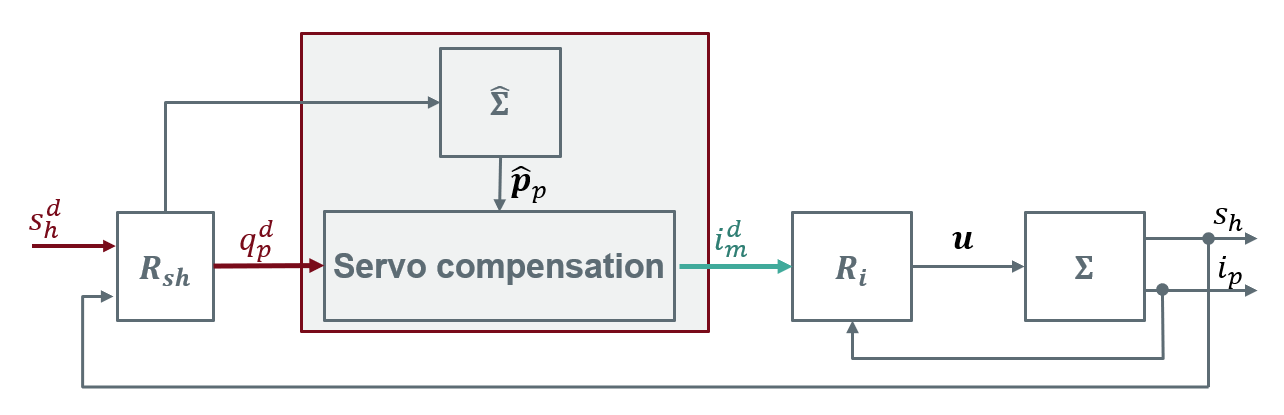
\includegraphics[width=0.8\columnwidth]{graphics/pgfplots/cha5/Bosch/blockschaltbild.png}
	\caption{Block diagram of the servo-compensation.}
	\label{fig:blockschaltbild}
\end{figure}

The data $\mathcal{D}$ consisting of 1000 points is generated using a validated model based on first-principles and visualized in Figure \ref{fig:bosch_data_situation}. The figure shows two distinct model regions with a discontinuity at the position $s_h = 0$. The main challenge here is to model the discontinuity in a smooth way without introducing modeling artifacts, i.e. over- or undershooting behavior. We know beforehand that the differential current $i_m^d$ is monotonic increasing with the differential flow $q_p^d$. We further constrain the models to be monotonic increasing with the differential flow $q_p^d$ to enforce a smooth transition at the discontinuity at $s_h = 0$.

\begin{figure}[H]
	\centering
	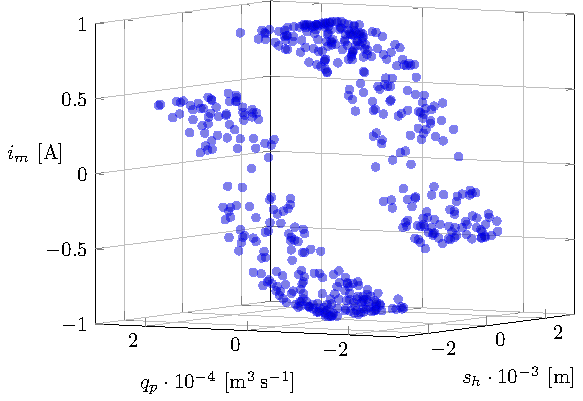
\includegraphics{graphics/pgfplots/cha5/Bosch/data_situation.pdf} 
	\caption{Data Situation}
	\label{fig:bosch_data_situation}
\end{figure}

We will now use various models based on B-spline bases, tensor-product B-spline bases and their shape-constraint alternatives to recover a model for the differential current $i_m^d$. The following list, in which $s(x_i)$ denotes the use of a B-spline basis for input $x_i \in \{q_p^d, s_h\}$ and $t(q_p^d, s_h)$ denotes the use of a tensor-product B-spline basis, describes the models that are analyzed.

\begin{enumerate}[(i)]
	\item M1 $= s(q_p^d) + s(s_h)$, without constraints
	\item M2 $= s(q_p^d) + s(s_h)$, with monotonicity for $s(s_h)$
	\item M3 $= t(q_p^d,s_h)$, without constraints
	\item M4 $= t(q_p^d,s_h)$, with monotonicity for input $s(q_p^d)$ and $s(s_h)$
	\item M5 $= s(s_h) + t(q_p^d,2)$, as additive model without constraints
	\item M6 $= s(s_h) + t(q_p^d,2)$, as additive model with the constraints defined in M2 and M4
\end{enumerate}
%
To fit the models listed above, we perform a randomized train-validation split on the data. The training set $\mathcal{D}_{\text{train}}$ then consists of 750 data points and a validation set $\mathcal{D}_{\text{val}}$ of 250 data points. We fit the models to the resulting training set and evaluate its performance by calculating the mean squared error on the validation set $\mathcal{D}_{\text{val}}$ and the effective degree of freedom of the models EDoF, as well as by visual inspection.

Note that we use a smoothness penalty optimized via generalized cross-validation for each individual basis. The unconstraint models M1, M3 and M5 are therefore P-spline models rather than B-spline models. The shape-constraint models M2, M4 and M6 are SCP-spline models. The mean squared errors $\mathrm{MSE}_{\mathrm{val}}$ evaluated on the validations set $\mathcal{D}_{\text{val}}$ are given in~\pref{tab:bosch-mse-val} as well as the effective degree of freedom of the models as a measure of the model complexity. 

\begin{table}[H]
	\begin{center}
		\pgfplotstabletypeset[
		col sep=comma,
		columns/Model/.style={string type},
		columns/MSE_val/.style={column name={$\text{MSE}_{\text{val}}$}},
		every head row/.style={before row=\toprule[1pt] \toprule,after row=\midrule[2pt]},
		every last row/.style={after row=\bottomrule \bottomrule},
		every nth row={1}{before row=\midrule},
		]{graphics/data/cha5/Bosch/mses.csv}
	\end{center}
	\caption{Mean squared errors on the validation set $\mathcal{D}_{\text{val}}$ and the effective degree of freedom $\text{EDoF}$ of the models.}
	\label{tab:bosch-mse-val}
\end{table}

The purely B-spline based models M1 and M2 show low degrees of freedom but higher values of the mean squared error on the validation set $\mathcal{D}_{\text{val}}$. Therefore, they lack some flexibility to model the data accurately. The predictions for these models are visualized in~\pref{fig:bosch-M1} and~\pref{fig:bosch-M2}. Note the left plot is the projection of the three dimensional data onto the $s_h$ axis for better visualization of the model predictions. The purely tensor-product B-spline models M3 and M4 have a significantly lower mean squared error on the validation set $\mathcal{D}_{\text{val}}$. Both models are visualized in~\pref{fig:bosch-M3} and~\pref{fig:bosch-M4}. With regards to the effective degree of freedom, we see that the regularization through the shape-constraints clearly decreases the model flexibility which leads to a better generalization behavior seen by the lower $\text{MSE}_{\text{val}}$ of M4 compared to M3. This can also be seen in the left plot of~\pref{fig:bosch-M3}. Note, for example, the prediction point (red) at $s_h \approx 0.7 \cdot 10^{-4}$. Such a prediction is only possible for a very wiggly and non-smooth function. The additive models using B-splines and tensor-product B-splines, i.e. M5 and M6, both show low mean squared errors on the validation set $\text{MSE}_{\text{val}}$. We again see the effect of the shape-constraint in the effective degree of freedom as well as in the plots in~\pref{fig:bosch-M5} and~\pref{fig:bosch-M6}. 

\begin{figure}[H]
	\centering 
	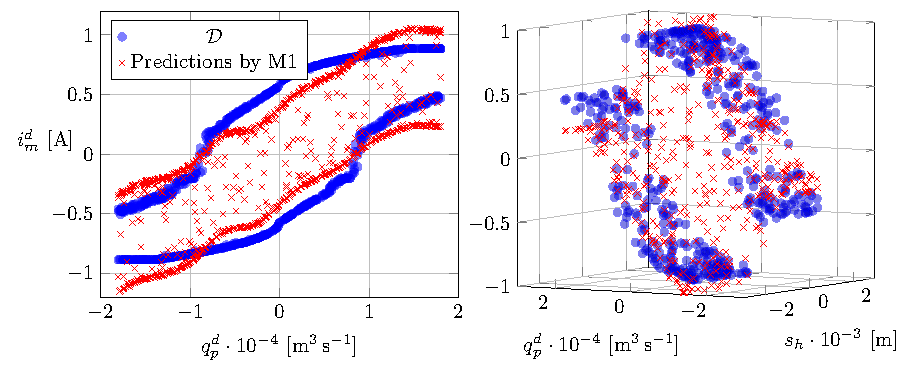
\includegraphics{graphics/pgfplots/cha5/Bosch/M1.pdf}
	\caption{Data $\mathcal{D}$ and predictions by model M1.}
	\label{fig:bosch-M1}
\end{figure}

\begin{figure}[H]
	\centering 
	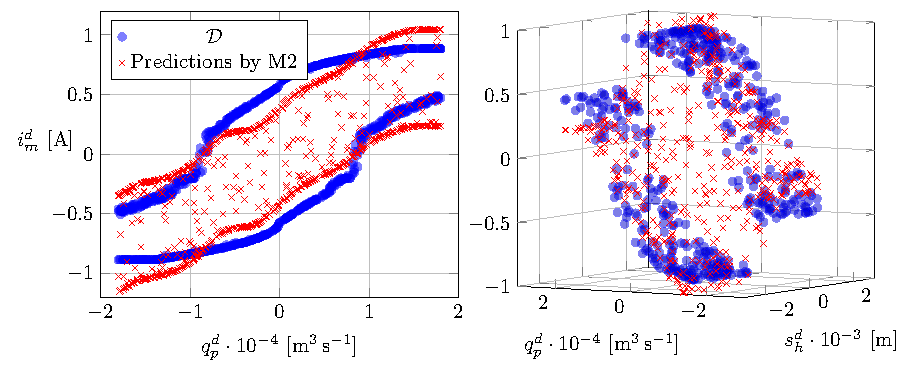
\includegraphics{graphics/pgfplots/cha5/Bosch/M2.pdf}
	\caption{Data $\mathcal{D}$ and predictions by model M2.}
	\label{fig:bosch-M2}
\end{figure}

\begin{figure}[H]
	\centering 
	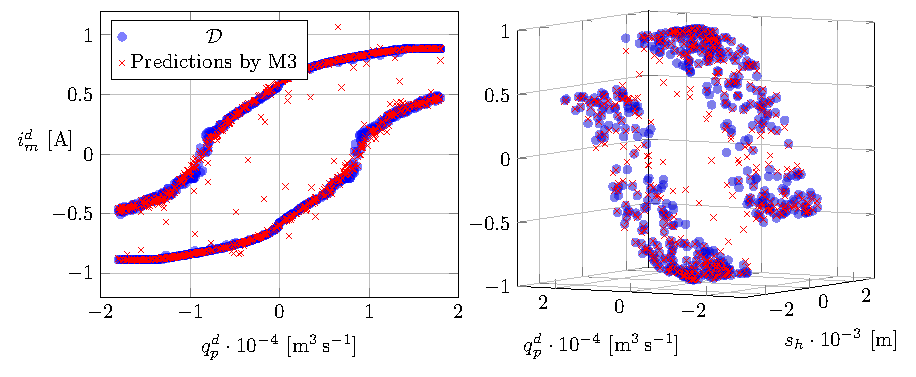
\includegraphics{graphics/pgfplots/cha5/Bosch/M3.pdf}
	\caption{Data $\mathcal{D}$ and predictions by model M3.}
	\label{fig:bosch-M3}
\end{figure}

\begin{figure}[H]
	\centering 
	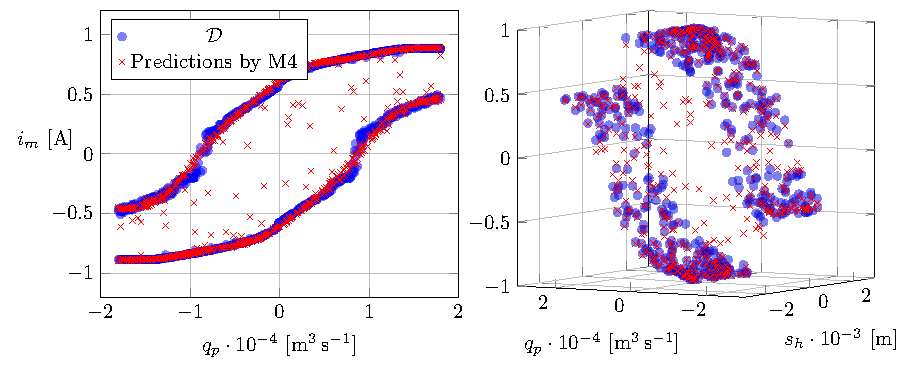
\includegraphics{graphics/pgfplots/cha5/Bosch/M4.pdf}
	\caption{Data $\mathcal{D}$ and predictions by model M4.}
	\label{fig:bosch-M4}
\end{figure}

\begin{figure}[H]
	\centering 
	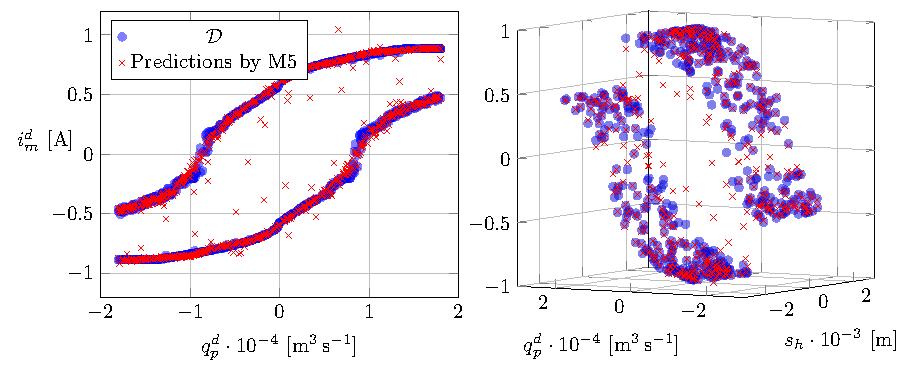
\includegraphics{graphics/pgfplots/cha5/Bosch/M5.pdf}
	\caption{Data $\mathcal{D}$ and predictions by model M5.}
	\label{fig:bosch-M5}
\end{figure}

\begin{figure}[H]
	\centering 
	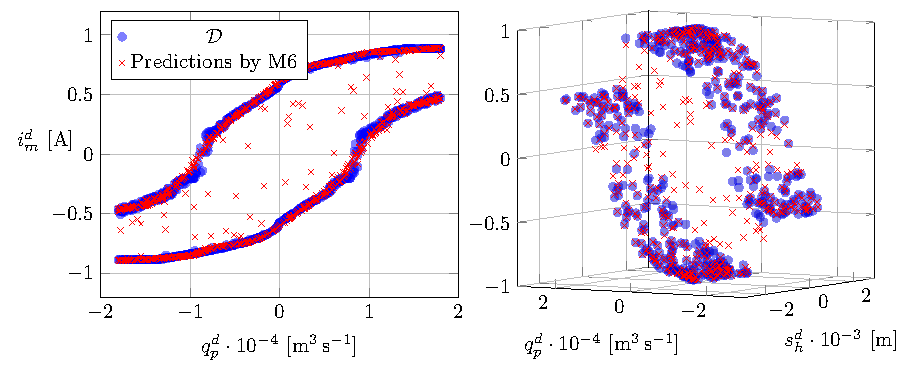
\includegraphics{graphics/pgfplots/cha5/Bosch/M6.pdf}
	\caption{Data $\mathcal{D}$ and predictions by model M6.}
	\label{fig:bosch-M6}
\end{figure}

To summarized, we see that the incorporation of a priori domain knowledge improves the quality of the fit for this example too. The constrained models show lower mean squared errors on the validation data as well as lower effective degrees of freedom. The best model is clearly M6, since it has a significantly lower $\text{MSE}_{\text{val}}$ as well as EDoF. 